\documentclass[12pt,twoside]{article}
\usepackage{amsmath, amssymb}
\usepackage{amsmath}
\usepackage[active]{srcltx}
\usepackage{amssymb}
\usepackage{amscd}
\usepackage{makeidx}
\usepackage{amsthm}
\usepackage{algpseudocode}
\usepackage{algorithm}
\usepackage{graphicx}
\usepackage[spanish, es-tabla]{babel}
\usepackage{multirow}
\renewcommand{\baselinestretch}{1}
\graphicspath{{images/}}
\setcounter{page}{1}
\setlength{\textheight}{21.6cm}
\setlength{\textwidth}{14cm}
\setlength{\oddsidemargin}{1cm}
\setlength{\evensidemargin}{1cm}
\pagestyle{myheadings}
\thispagestyle{empty}
\markboth{\small{Pr\'actica 5. Alan, Josu\'e}}{\small{.}}
\date{}
\begin{document}
\centerline{\bf An\'alisis de Algoritmos, Sem: 2020-1, 3CV2, Pr\'actica 5, 25 de septiembre}
\centerline{}
\centerline{}
\begin{center}
\Large{\textsc{Pr\'actica 5}}
\end{center}
\centerline{\bf{Alan Romero Lucero, Josu\'e David Hern\'andez Ram\'irez}}
\centerline{}
\centerline{Escuela Superior de C\'omputo}
\centerline{Instituto Polit\'ecnico Nacional, M\'exico}
\centerline{$alanrl.escom@gmail.com, josuehernandezr082@gmail.com$}
\newtheorem{Theorem}{\quad Theorem}[section]
\newtheorem{Definition}[Theorem]{\quad Definition}
\newtheorem{Corollary}[Theorem]{\quad Corollary}
\newtheorem{Lemma}[Theorem]{\quad Lemma}
\newtheorem{Example}[Theorem]{\quad Example}
\bigskip
\textbf{Resumen:} En el desarrollo de esta pr\'actica se hace comparaci\'on de tres algoritmos de ordenamiento, el \textit{shell-sort}, \textit{cocktail-sort} y \textit{heap-sort}.
{\bf Palabras Clave:} {\textit{algoritmo, ordenamiento, arbol, bubble-sort, insertion-sort}}
\section{Introducci\'on}
Hay algoritmos de ordenamiento que son ampliamente famosos como el \textit{bubble, merge o quick sort}, sin embargo, hay muchos otros algoritmos interesantes que valen la pena ser analizados y comprender su funcionamiento. Entre estos, se analizaran los algoritmos \textit{shell-sort, cocktail-sort y heap sort}, los cuales ser\'an comparados entre s\'i, en sus mejores y peores casos. Estos algoritmos tambi\'en son conocidos, sin embargo no son tan comunmente mencionados como el \textit{quick o merge}, adem\'as, su complejidad no es difiere mucho de las complejidades que se han estudiado previamente, no obstante su importancia no debe ser olvidada como una forma de ver como analizando otros algoritmos como el \textit{buble e insertion} se pueden desarrollar variaciones que den mejores resultados en promedio o den otros beneficios.

\section{Conceptos B\'asicos}
\subsection{Complejidad te\'orica de los algoritmos}
\begin{table}[htbp]
\centering
\begin{tabular}{|c|c|c|c|}
\hline
Algoritmo & Mejor caso & Caso Aleatorio & Peor caso \\
Heap-Sort & O(n log(n)) & O(n log(n)) & O(n log(n)) \\
Cocktail-Sort & O(n) & O(n\textasciicircum{}2) & O(n\textasciicircum{}2) \\
Shell-Sort & O(n) & O(n\textasciicircum{}3/2) or O(n log\textasciicircum{}2 (n)) & O(n\textasciicircum{}3/2) or O(n log\textasciicircum{}2 (n))
\end{tabular}
\caption{Tabla de complejidad te\'orica}
\end{table}
\subsection{\textit{Cockatil-Sort}}
El \textit{cocktail-sort} es una variaci\'on del bien conocido \textit{bubble-sort}. Para explicar este algoritmo primero hace falta explicar rapidamente el algoritmo burbuja. El algoritmo burbuja va recorriendo el arreglo que ser\'a ordenado desde la izquierda hacia la derecha, enviando el valor m\'as grande hasta el final. Asi con la primer iteracion, la segunda, etc.
\begin{figure}
    \centering
    \begin{equation}
        [ \longrightarrow 3,0,5,6,7,2]
    \end{equation}
    \begin{equation}
        [3,0,5,6,2,\longrightarrow 7]
    \end{equation}
    \begin{equation}
        \dots
    \end{equation}
    \caption{Funcionamiento del algoritmo burbuja}
    \label{eq:bubble_sort}
\end{figure}
Ahora el \textit{cocktail-sort} esta dividido en dos pasos. Hace una primer iteracion, en la recorre el arreglo desde la izquierda a la derecha, llevando el valor m\'as grande hasta el final del arreglo. Posteriormente, se recorre el arreglo de derecha a izquierda, llevando el menor valor hasta el inicio del arreglo, ordenandolo al finalizar. El algoritmo se detiene si al recorrer el arreglo no hizo ningun intercambio entre los elementos.
\begin{figure}[h]
    \centering
    \begin{equation}
        [ \longrightarrow 3,0,5,6,7,2]
    \end{equation}
    \begin{equation}
        [3,0,5,6,2,\longrightarrow 7]
    \end{equation}
    \begin{equation}
        [3,0,5,6,2,7 \longleftarrow]
    \end{equation}
    \begin{equation}
        [0 \longleftarrow ,3,5,6,2,7]
    \end{equation}
    \begin{equation}
        [ \longrightarrow 0,3,5,6,2,7]
    \end{equation}
    \begin{equation}
        [0,3,5,2,\longrightarrow 6,7]
    \end{equation}
    \begin{equation}
        [0,3,5,2,6,7 \longleftarrow]
    \end{equation}
    \begin{equation}
        [0,2 \longleftarrow ,3,5,6,7]
    \end{equation}
    \begin{equation}
        [ \longrightarrow 0,2,3,5,6,7]
    \end{equation}
    \begin{equation}
        [ 0,2,3,5,6,7 \longrightarrow]
    \end{equation}
    \caption{Ejemplo de cocktail-sort}
    \label{eq:cocktail}
\end{figure}
Es evidente su parecido con el algoritmo burbuja, sin embargo, tambi\'en se entiende claramente la idea que plantea este algoritmo y su diferencia.
\subsection{\textit{Shell-Sort}}
De manera analoga al \textit{cocktail-sort}, el \textit{shell-sort} es una variacion de otro algoritmo de ordenamiento, en este caso del \textit{insertion-sort}. A diferencia del algoritmo previamente mencionado, el \textit{shell-sort} hace comparaciones entre elementos que no estan juntos, lo que permite hacer intercambios entre elementos que estan distante entre s\'i.
A continuacion se ejemplifica su funcionamiento y su pseudo codigo para su mejor comprensi\'on.
\begin{algorithmic}
\Procedure{shell}{A = [\dots, n]}
    \For{$gap \longleftarrow \frac{n}{2} \text{ to } gap > 0, gap \longleftarrow \frac{gap}{2}$}
        \For{$ i \longleftarrow gap \text{ to } n$}
            \State $tmp \longleftarrow A[i]$
            \For{$j \longleftarrow i \text{ to } j >= gap \text{ and } A[j - gap] > tmp$}
                \State $A[j] \longleftarrow A[j - gap]$
            \EndFor
            \State $A[j] \longleftarrow tmp$
        \EndFor
    \EndFor
\EndProcedure
\end{algorithmic}
\begin{figure}[h]
    \centering
    \begin{equation}
        2,4,8,1,0 \longleftarrow \text{Arreglo original}
    \end{equation}
    \begin{equation}
        2,4,[tmp \longleftarrow 8],1,0 \longleftarrow \text{A la mitad, gap = 2}
    \end{equation}
    \begin{equation}
        2,4,[8],1,0 \longleftarrow \text{2 o 4 son menores que 8}
    \end{equation}
    \begin{equation}
        2,4,8,[tmp \longleftarrow 1],0 \longleftarrow \text{Ahora en i = 3}
    \end{equation}
    \begin{equation}
        2 , [1] , 8 , [4] , 0  \longleftarrow \text{Se intercambia el 3 y el 3 - 2 = 1}
    \end{equation}
    \begin{equation}
        1 , 4 , 8 , 2 , [tmp \longleftarrow 0]  \longleftarrow \text{Ahora i = 4}
    \end{equation}
    \begin{equation}
        1 , 4 , [0] , 2 , [8]  \longleftarrow \text{Se intercambian los valores en 4 y 4 - 2 = 2}
    \end{equation}
    \begin{equation}
        [0] , 4 , [1] , 2 , 8  \longleftarrow \text{Se intercambian los valores en 2 y 2 - 2 = 0}
    \end{equation}
    \begin{equation}
        0 , [4] , 1 , 2 , 8  \longleftarrow \text{Ahora gap es 1 y 0 < 4}
    \end{equation}
    \begin{equation}
        0 , 4 , [1] , 2 , 8  \longleftarrow \text{Ahora i = 2}
    \end{equation}
    \begin{equation}
        0 , [1] , [4] , 2 , 8  \longleftarrow \text{Se intercambian los valores en 2 y en 2 - 1 = 1}
    \end{equation}
    \begin{equation}
        0 , 1 , 4 , [2] , 8  \longleftarrow \text{ Ahora i = 3}
    \end{equation}
    \begin{equation}
        0 , 1 , [2] , [4] , 8  \longleftarrow \text{Se intercambian los valores en 3 y 3 - 1 = 2}
    \end{equation}
    \begin{equation}
        0 , 1 , 2 , 4 , [8]  \longleftarrow \text{Ahora i = 4}
    \end{equation}
    \begin{equation}
        0 , 1 , 2, 4, 8  \longleftarrow \text{El siguiente gap es igual a 0, el arreglo esta ordenado}
    \end{equation}
    \caption{Algoritmo shell-sort en funcionamiento}
    \label{eq:shell}
\end{figure}
\subsection{\textit{Heap-Sort}}
Este algoritmo esta basado en la estructura de datos \'arbol binario especial, que tiene la caracter\'istica que cada nodo tiene un valor superior al valor de sus hijos (\textit{binary heap}). El algoritmo construye un \'arbol binario. Posterior mente se acomoda con las caracter\'istica anteriores. Se tiene la ra\'iz, y si uno de sus dos hijos mayor, se intercambian entre s\'i. Esto se repite de manera recursiva hasta que cada nodo cumple la caracter\'istica mencionada al principio. Esto se repite hasta que se obtiene el valor m\'aximo, el cual se intercambia con el elemento final del arreglo. El siguiente \'arbol ya no tendr\'a el elemento acomodado y esto se repetir\'a hasta que solo queda un elemento, momento en el que el arreglo quedar\'a ordenado.

\section{Experimentaci\'on y Resultados}
Todo la explicación te\'orica y pseudoc\'odigo no tiene importancia si no se muestra su funcionamiento.

\\En esta secci\'on se mostrará la salida de la consola de los algoritmos antes mencionados y tambi\'en trazaremos la complejidad de cada uno en su mejor, aleatorio y peor caso.

\subsection{Algoritmo Heap-Sort}
En esta prueba, el programa trazará el tiempo que tarda el algoritmo en ordenar tres listas de tamaño n = 50.
La primera lista tendrá los elementos ya ordenados, la segunda tendrá los elementos en orden aleatorio y la tercera lista tendr\'a los elementos ordenados pero en orden decreciente.

\begin{figure}{h}
    \centering
    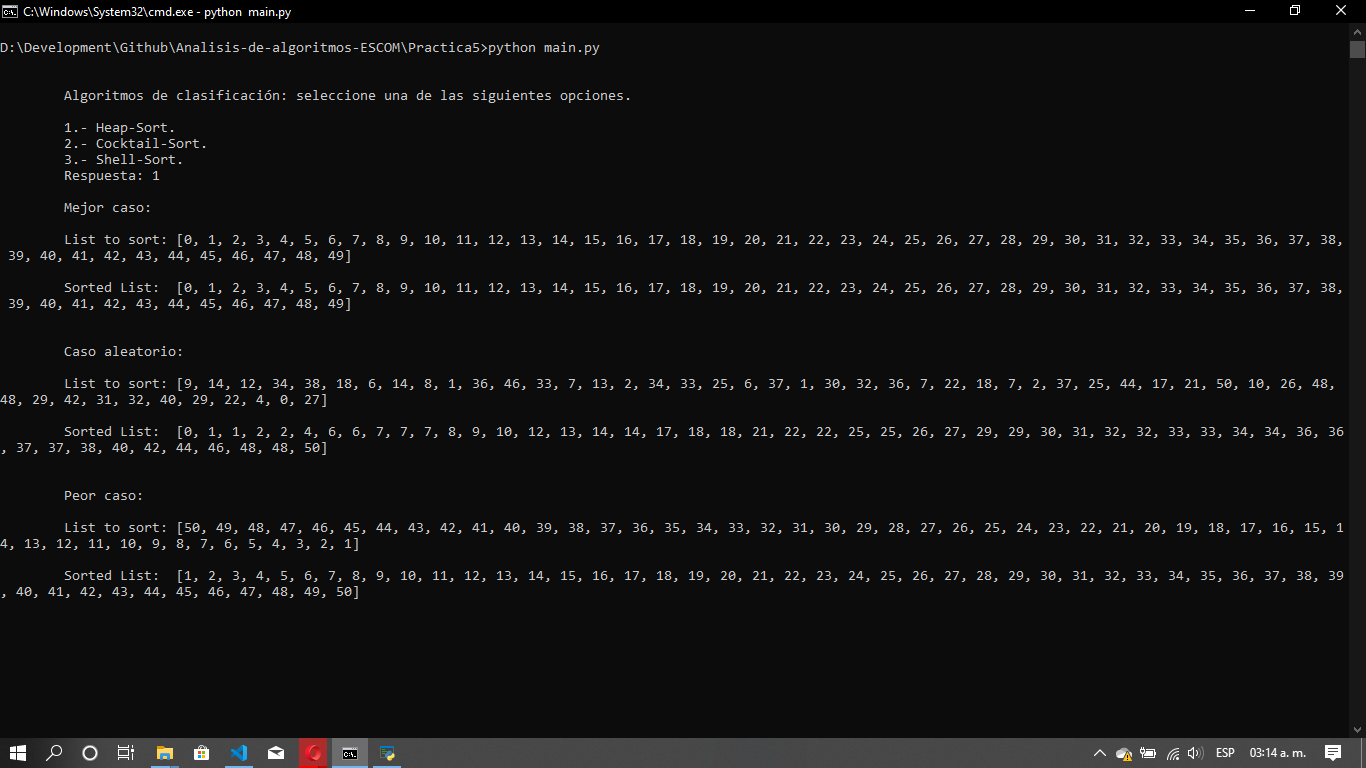
\includegraphics[width=13cm, height=8cm]{HeapConsole.png}
    \caption{Programa del algoritmo HeapSort en ejecuci\'on}
    \label{fig:quick_program}
\end{figure}

\begin{figure}{h}
    \centering
    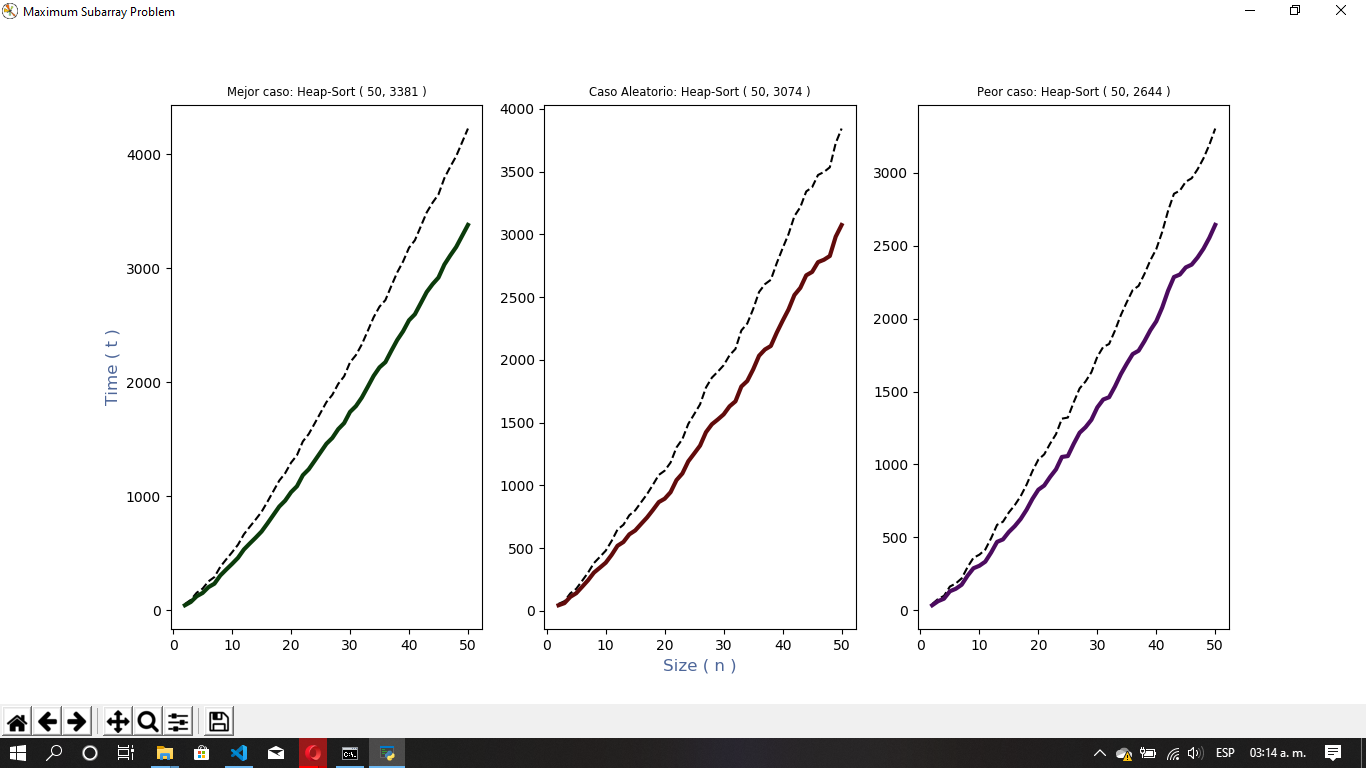
\includegraphics[width=13cm, height=8cm]{HeapGraph.png}
    \caption{Gr\'aficas de los casos del algoritmo HeapSort}
    \label{fig:quick_program}
\end{figure}
\\\\
Así es como podemos observar, en todas las gr\'aficas se cumple el orden de complejidad pero, variando en el tiempo en que tarda y por ende, el "ruido" que existe en las gr\'aficas.
\subsection{Algoritmo Cocktail-Sort}
En esta prueba, el programa trazará el tiempo que tarda el algoritmo en ordenar tres listas de tamaño n = 50.
La primera lista tendrá los elementos ya ordenados, la segunda tendrá los elementos en orden aleatorio y la tercera lista tendr\'a los elementos ordenados pero en orden decreciente.
\begin{figure}{h}
    \centering
    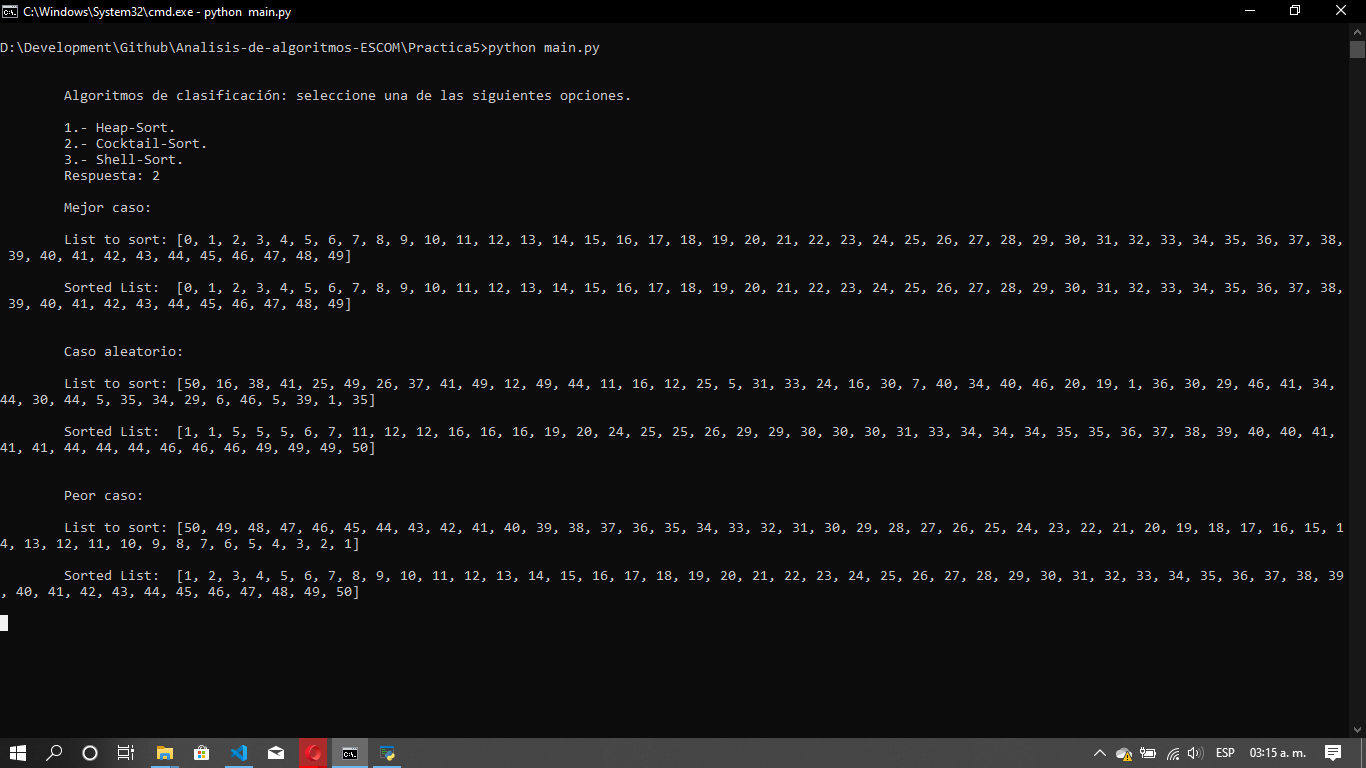
\includegraphics[width=13cm, height=8cm]{CocktailConsole.png}
    \caption{Programa del algoritmo CocktailSort en ejecuci\'on}
    \label{fig:quick_program}
\end{figure}
\begin{figure}{h}
    \centering
    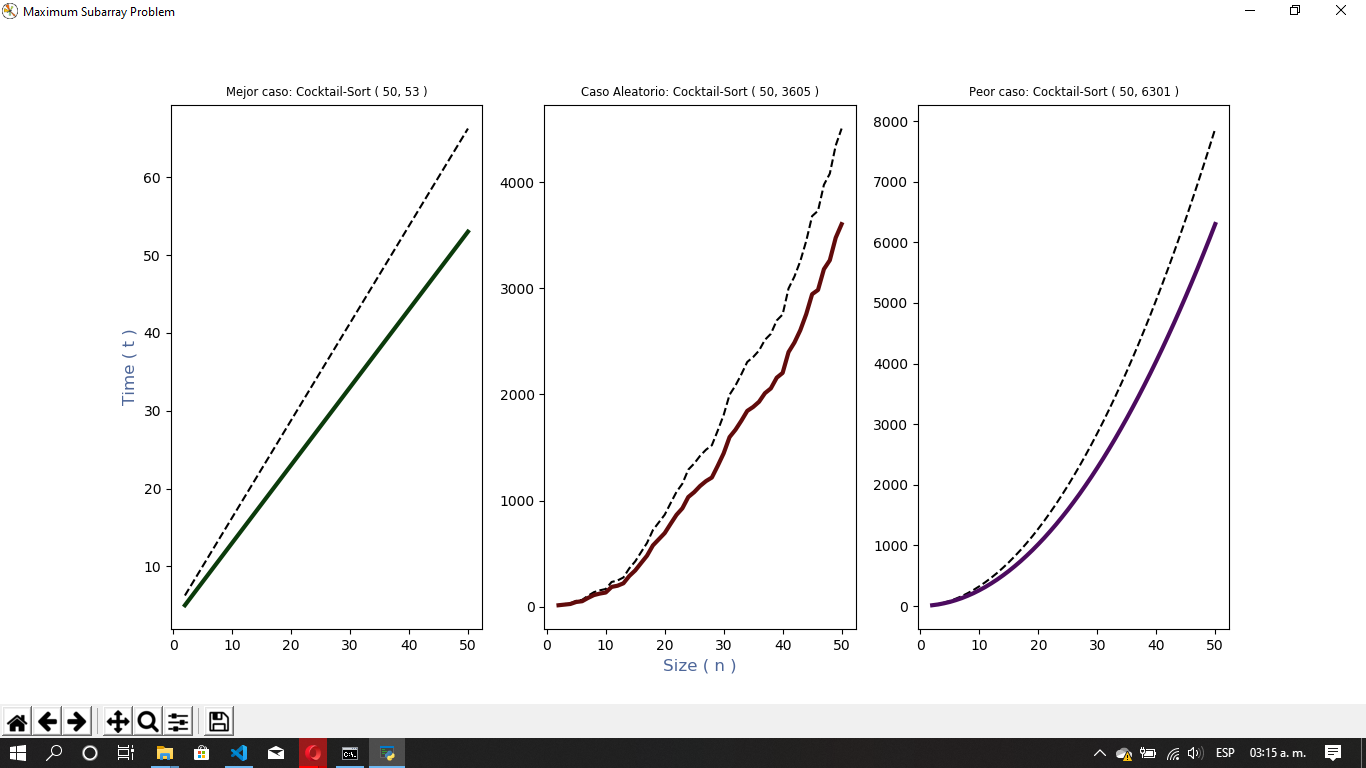
\includegraphics[width=13cm, height=8cm]{CocktailGraph.png}
    \caption{Gr\'aficas de los casos del algoritmo CocktailSort}
    \label{fig:quick_program}
\end{figure}

\\
As\'i es como podemos reiterar que las complejidades que tiene el algoritmo, visto en la secci\'on 2, se cumple bien, ya que en su mejor caso todo es lineal y en su peor se cumple que es cuadr\'atica.

\subsection{Algoritmo Shell-Sort}
En nuestra ultima prueba para este algoritmo, consiste en trazar la complejidad de las listas de tamaño n = 50, con esto nos damos a la idea de que en el mejor caso, esta muy cerca de ser lineal.

\begin{figure}{h}
    \centering
    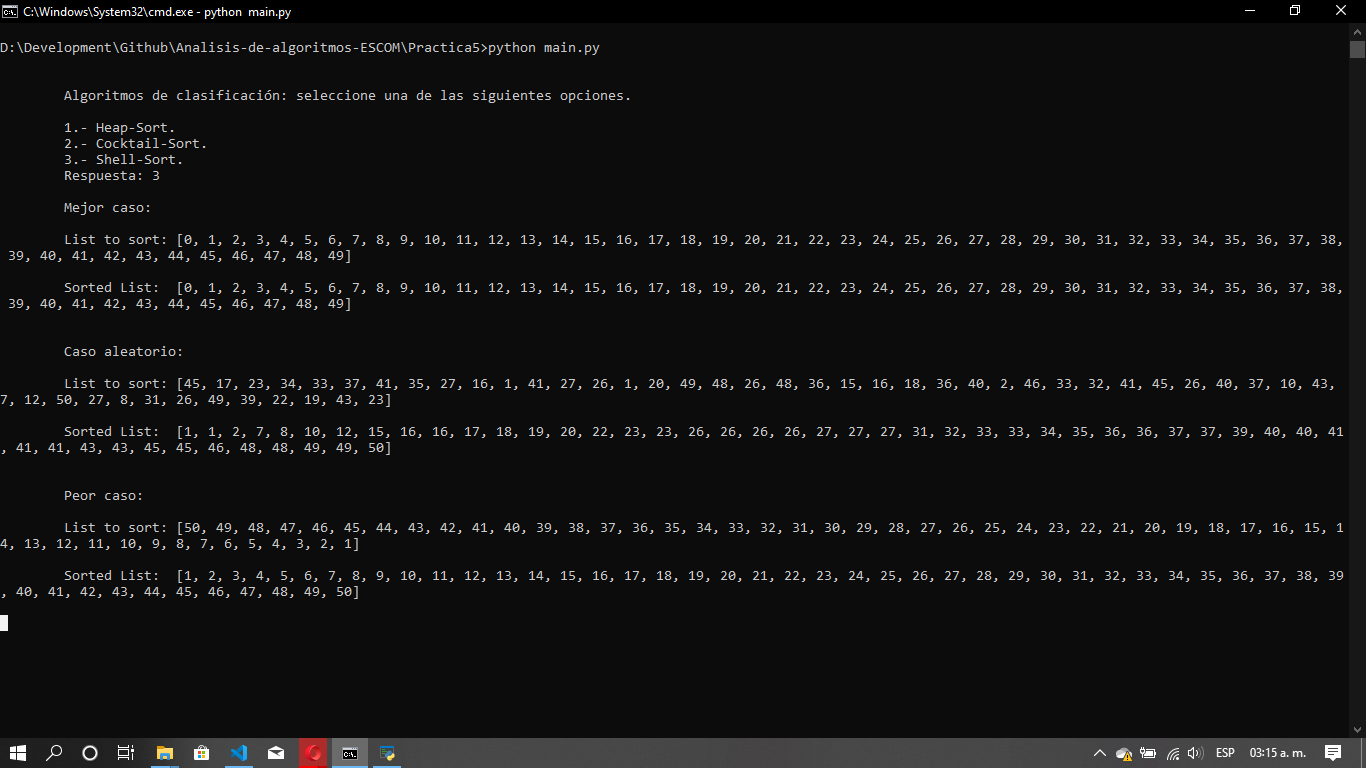
\includegraphics[width=13cm, height=8cm]{ShellSortConsole.png}
    \caption{Programa del algoritmo ShellSort en ejecuci\'on}
    \label{fig:quick_program}
\end{figure}

\begin{figure}{h}
    \centering
    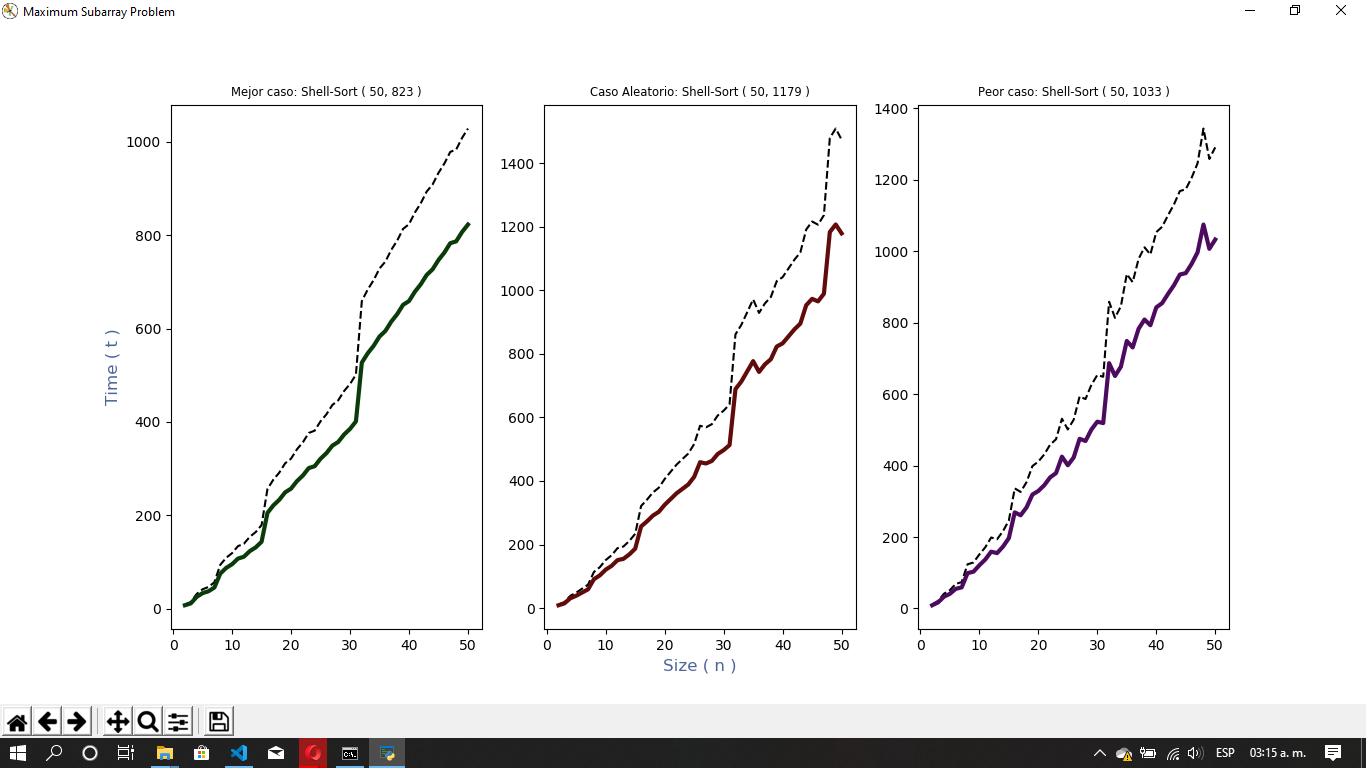
\includegraphics[width=13cm, height=8cm]{ShellSortGraph.png}
    \caption{Gr\'aficas de los casos del algoritmo ShellSort}
    \label{fig:quick_program}
\end{figure}
\\\\




\section{Conclusiones}

\textit{Alan Romero Lucero}. Podemos que dos de los tres algoritmos son derivaciones de otros algoritmos de ordenamiento, dados gracias al an\'alisis de estos. El caso del cocktail-sort no lo veo muy practico, ya que tanto en su peor como en su caso promedio tiene complejidad $n^2$ por lo que no le diferencia o practicidad contra el algoritmo burbuja, aunque su implementaci\'on depender\'a del caso y seguramente habr\'a casos que es mejor que burbuja, sin embargo, no lo considero muy relevante contra casos promedio. Se puede considerar un caso similar al shell-sort cuya complejidad en el peor caso es $\mathcal{O}(n)$. Sin embargo, en este algoritmo se pueden tener diferentes implementaciones al seleccionar el \textit{gap} que permiten reducir su complejidad, por lo que encuentro mayor sentido a esta variaci\'on del insertion-sort. El heap-sort me resulta mas interesante debido a su utilizacion de un \'arbol binario para el ordenamiento, \'ademas de su complejidad $\mathcal{O}(n\log_2 n)$.


\textit{Josu\'e David Hern\'andez Ram\'irez}. Ademas de su complejidad para graficar los resultados, es importante saber que otros algoritmos de ordenaci\'on existen, y que estos pueden ser estables o no estables, y que puede afectar a los resultados, ya que en estos algoritmos los casos promedio son los que suceden mas a menudo y por ende se toma su complejidad promedio como la verdadera. Sin embargo a veces es mas \'optimo usar otros algoritmos a los que son mas estables o eficientes y esto depende de cada tarea que se vaya a realizar, ya que al usar algoritmos no estables, puedes obtener mas poder de procesamiento, o que este mismo en comparaci\'on a otros no consuma recursos innecesarios, haciendo mas eficiente su uso.
\newpage
\vfill
\clearpage
\section{Bibliograf\'ia}
\newline
GeeksforGeeks. (2019). Cocktail Sort - GeeksforGeeks. [online] Available at: https://www.geeksforgeeks.org/cocktail-sort/ [Accessed 25 Sep. 2019].
\newline\newline
GeeksforGeeks. (2019). Shell Sort - GeeksforGeeks. [online] Available at:
\newline
https://www.geeksforgeeks.org/shellsort/ [Accessed 25 Sep. 2019].
\newline\newline
GeeksforGeeks. (2019). Heap Sort - GeeksforGeeks. [online] Available at:
\newline
https://www.geeksforgeeks.org/heap-sort/ [Accessed 25 Sep. 2019].
\end{document}